\documentclass{article}


\usepackage{PRIMEarxiv}
\usepackage[utf8]{inputenc} % allow utf-8 input
\usepackage[T1]{fontenc}    % use 8-bit T1 fonts
\usepackage{hyperref}       % hyperlinks
\usepackage{url}            % simple URL typesetting
\usepackage{booktabs}       % professional-quality tables
\usepackage{amsfonts}       % blackboard math symbols
\usepackage{nicefrac}       % compact symbols for 1/2, etc.
\usepackage{microtype}      % microtypography
\usepackage{lipsum}
\usepackage{fancyhdr}       % header
\usepackage{multicol}
\usepackage{graphicx}       % graphics
\usepackage{authblk}
\usepackage{float}
\usepackage{amsmath}
\graphicspath{{media/}}     % organize your images and other figures under media/ folder

\pagestyle{fancy}
\thispagestyle{empty}
\rhead{ \textit{ }} 

% Update your Headers here
\fancyhead[LO]{Analyze Influencing Factors of COVID-19 with R Language and Machine Learning Models}
% \fancyhead[RE]{Firstauthor and Secondauthor} % Firstauthor et al. if more than 2 - must use \documentclass[twoside]{article}

%% Title
\title{Analyze Influencing Factors of COVID-19 with \\R Language and Machine Learning Models
%%%% Cite as
%%%% Update your official citation here when published 
}

\author{Suizhi Ma\thanks{Algorithm Engineer}}
\author{Yuxing Pei\thanks{Test Engineer}}
\author{Ming Wang\thanks{Algorithm Engineer}}
\author{Longling Geng\thanks{Leader, Report Writter}}
\author{Jiaming Han\thanks{Data Engineer}}
\author{Yunfei Liu\thanks{Systems Architect, Report Writter}} 
\affil{Department of Computing, The Hong Kong Polytechnic University}

\renewcommand*{\Affilfont}{\small\it} 
\renewcommand\Authands{ and } 
\date{}

\begin{document}
\maketitle


\begin{abstract}
We have analyzed possible economical, political, and medical factors which may affect the spread of COVID-19 with R language and several machines learning regression models including multivariate linear regression and multivariate polynomial regression. Comparisons are made between countries and in countries to figure out the possible influencing factor’s effect on daily new confirmed cases. According to the result of our training models, political and economic factors may be more important in some aspects than vaccines.
\end{abstract}


% keywords can be removed
\keywords{COVID-19 \and Machine Learning \and R Language \and Data Analysis}

\begin{multicols}{2}

\section{Introduction}

\begin{figure}[H]
    \centering
    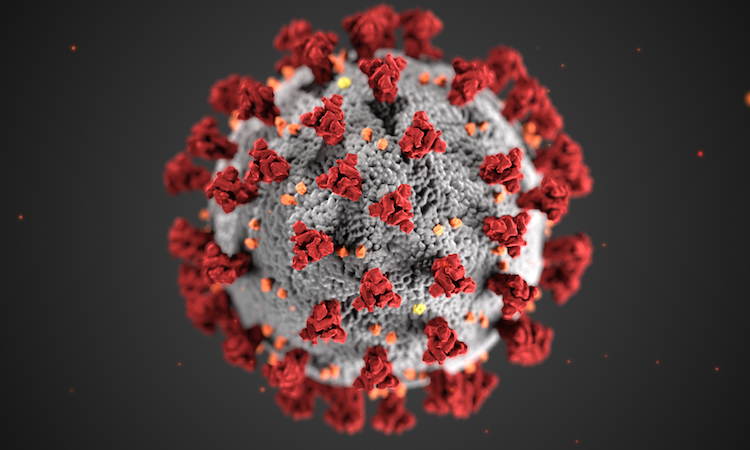
\includegraphics[width=0.45\textwidth]{covid.png}
    \caption{COVID-19}
    \label{fig:graph0}
\end{figure}

COVID-19 has received concern from the whole world, and people from the whole world are fighting against the epidemic together. To understand the spread of the virus, the human must figure out what factors affect the spreading speed. As global citizens, we feel that we should undertake the responsibility to make a contribution to the fight against the virus, and we are eager to implement what we have learned in this subject to achieve this target. In this project, we try to find what can affect the virus and the relation between spread speed and possible factors \cite{roser2020coronavirus}.

\begin{figure}[H]
    \centering
    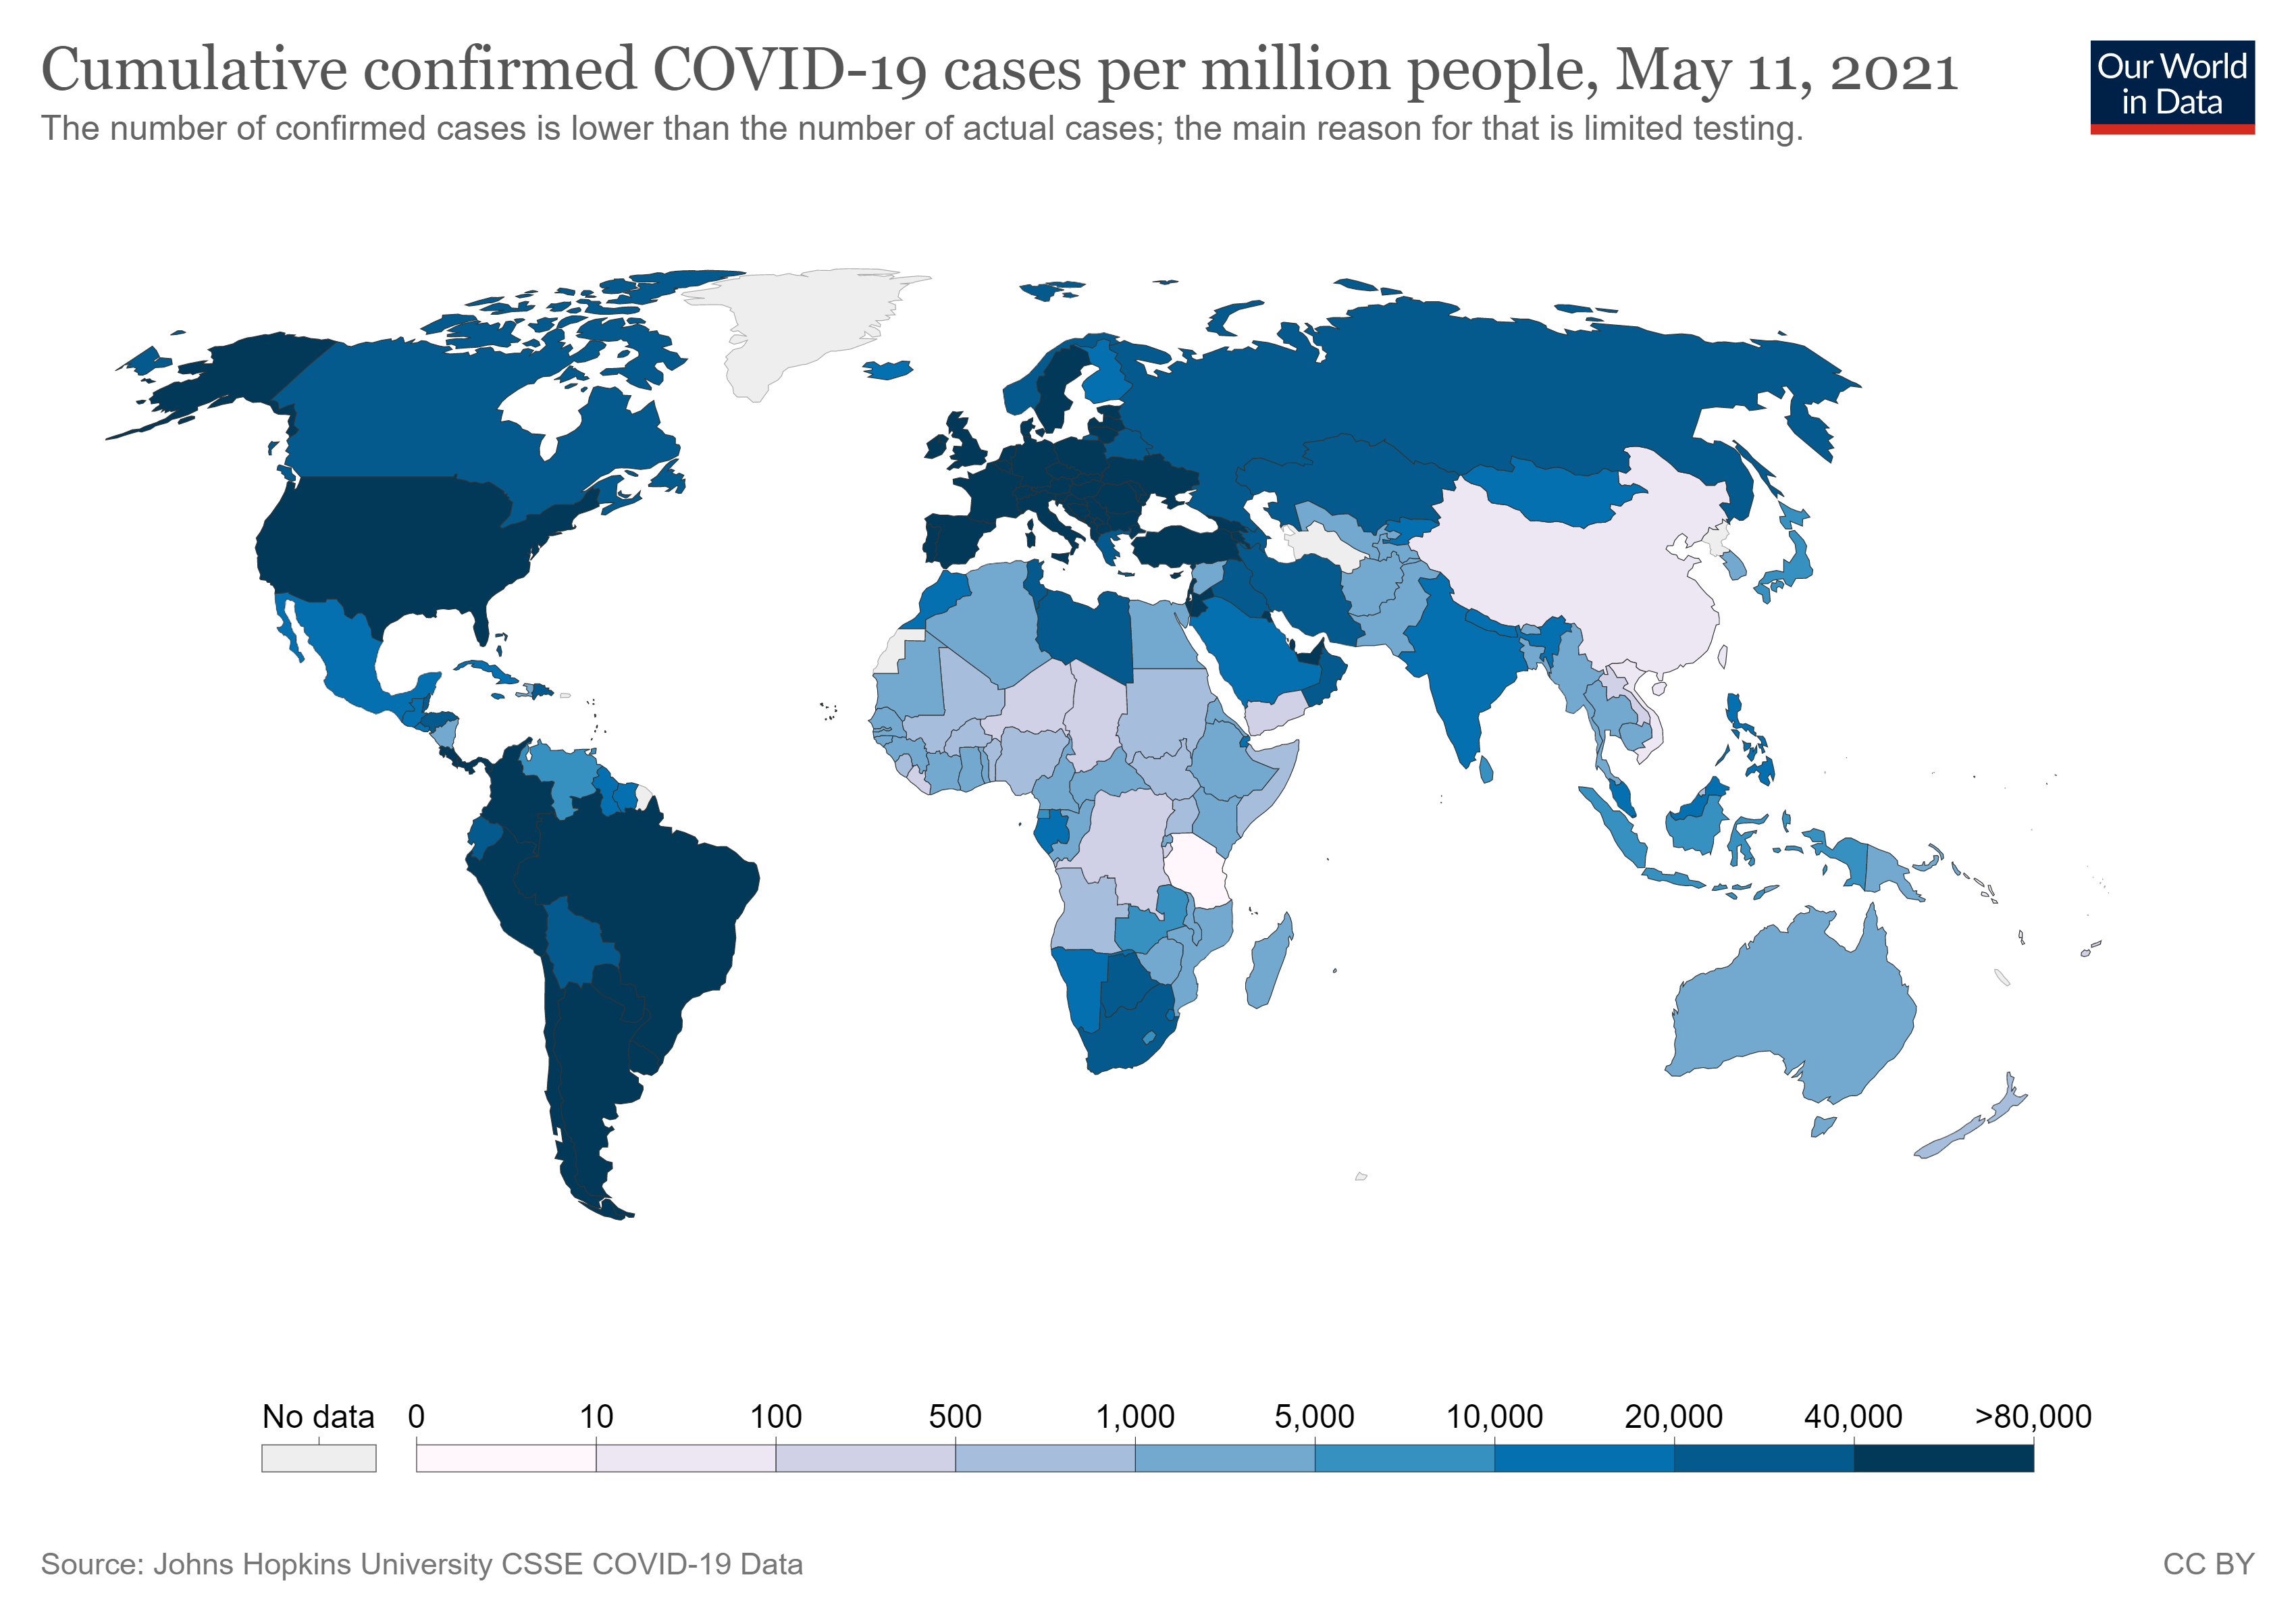
\includegraphics[width=0.45\textwidth]{totalconfirmed.png}
    \caption{Total confirmed COVID-19 cases in the world}
    \label{fig:graph1}
\end{figure}

\section{Motivation}
The very first intuition we choose the topic "Data analysis on the influencing factors of development of Covid-19" is deep interest. There is a large number of people in Kong Kong starting to take the vaccine \cite{tam2020impact}. Some people do not know much about the effectiveness of the vaccine. Some people are questioning the effectiveness. Therefore, as a group of students who are interested in the facts and truths behind the vaccine. We have a strong desire to find out the real impact of the vaccine \cite{kwok2020community}.

\begin{figure}[H]
    \centering
    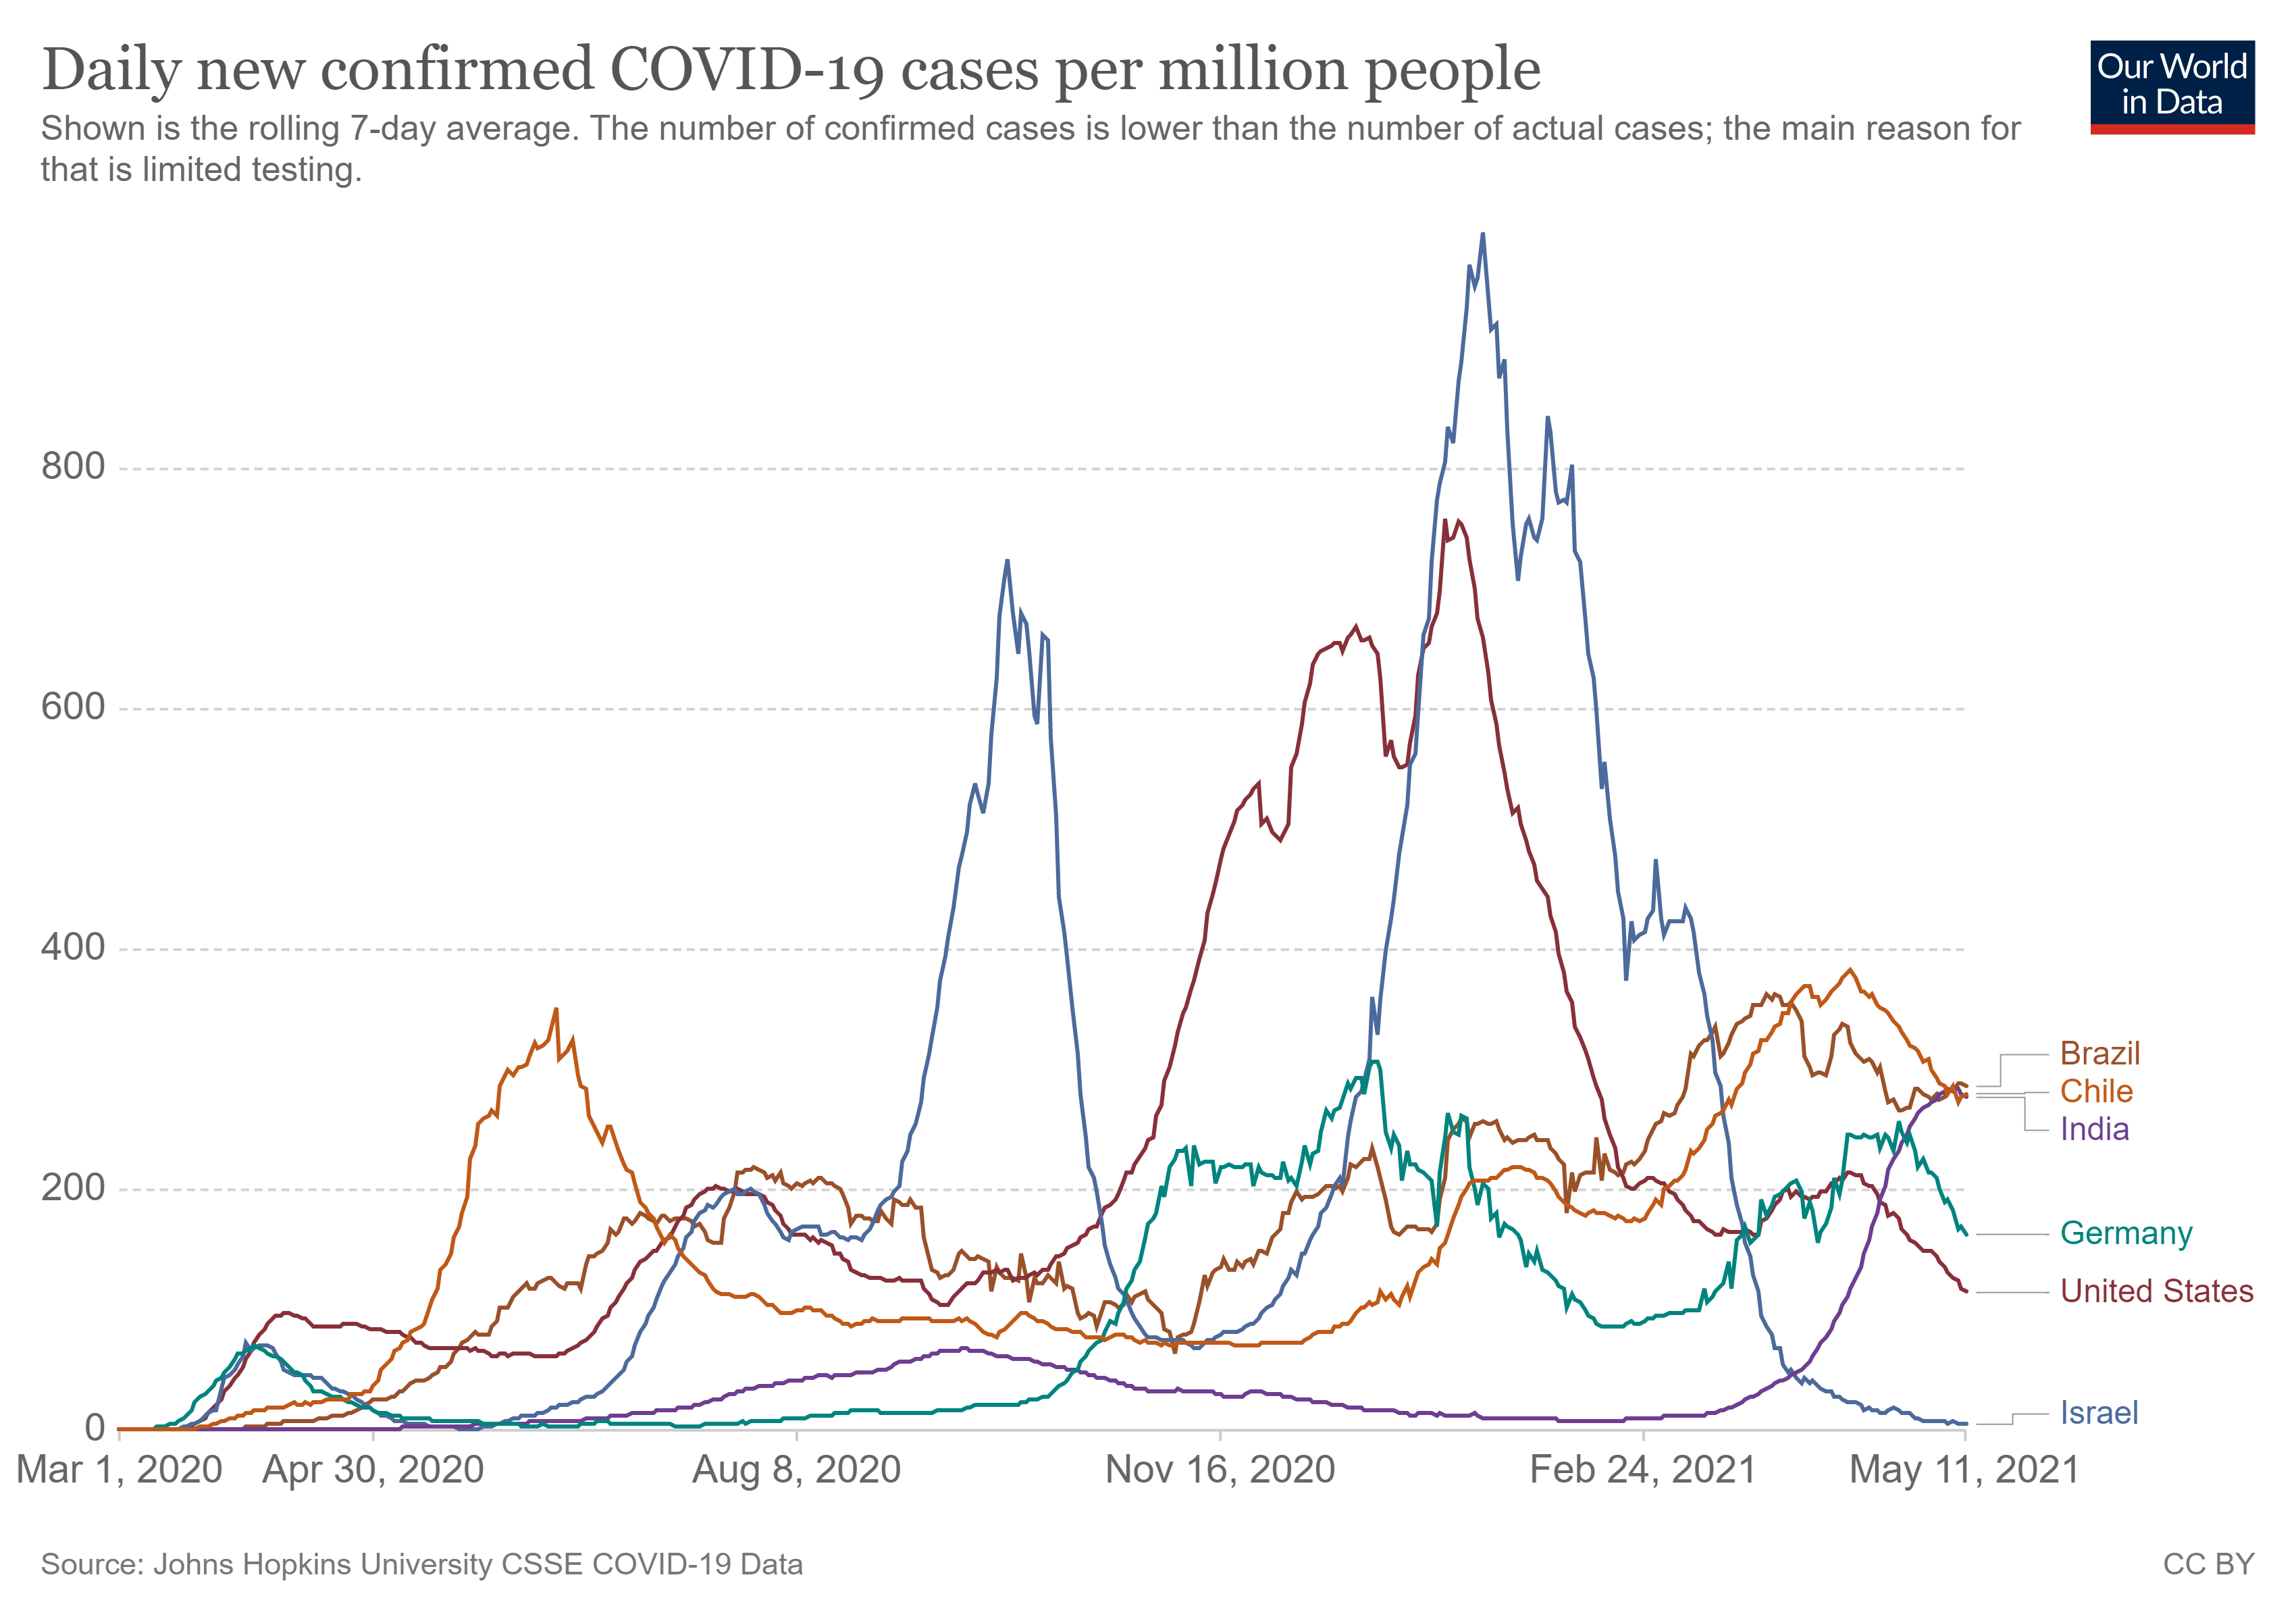
\includegraphics[width=0.45\textwidth]{newconfirmedpermillion.png}
    \caption{Confirmed COVID-19 cases fluctuation in some countries}
    \label{fig:graph2}
\end{figure}

However, before scientific research is conducted, only interest is not enough. The research topic should be proved valuable and worthy to discuss. After looking into various papers, we find out that theoretical value and reality research are two main issues that should be taken into consideration. On the theoretical side, a large number of related papers can be found and "Covid-19" and "related vaccine" are both the hot keywords in the academic library. On the reality side, this topic is proven to be useful because its result will benefit the government and the healthcare organization to take the measurement. Also, this topic is close to the hot and crucial social issue nowadays.

\begin{figure}[H]
    \centering
    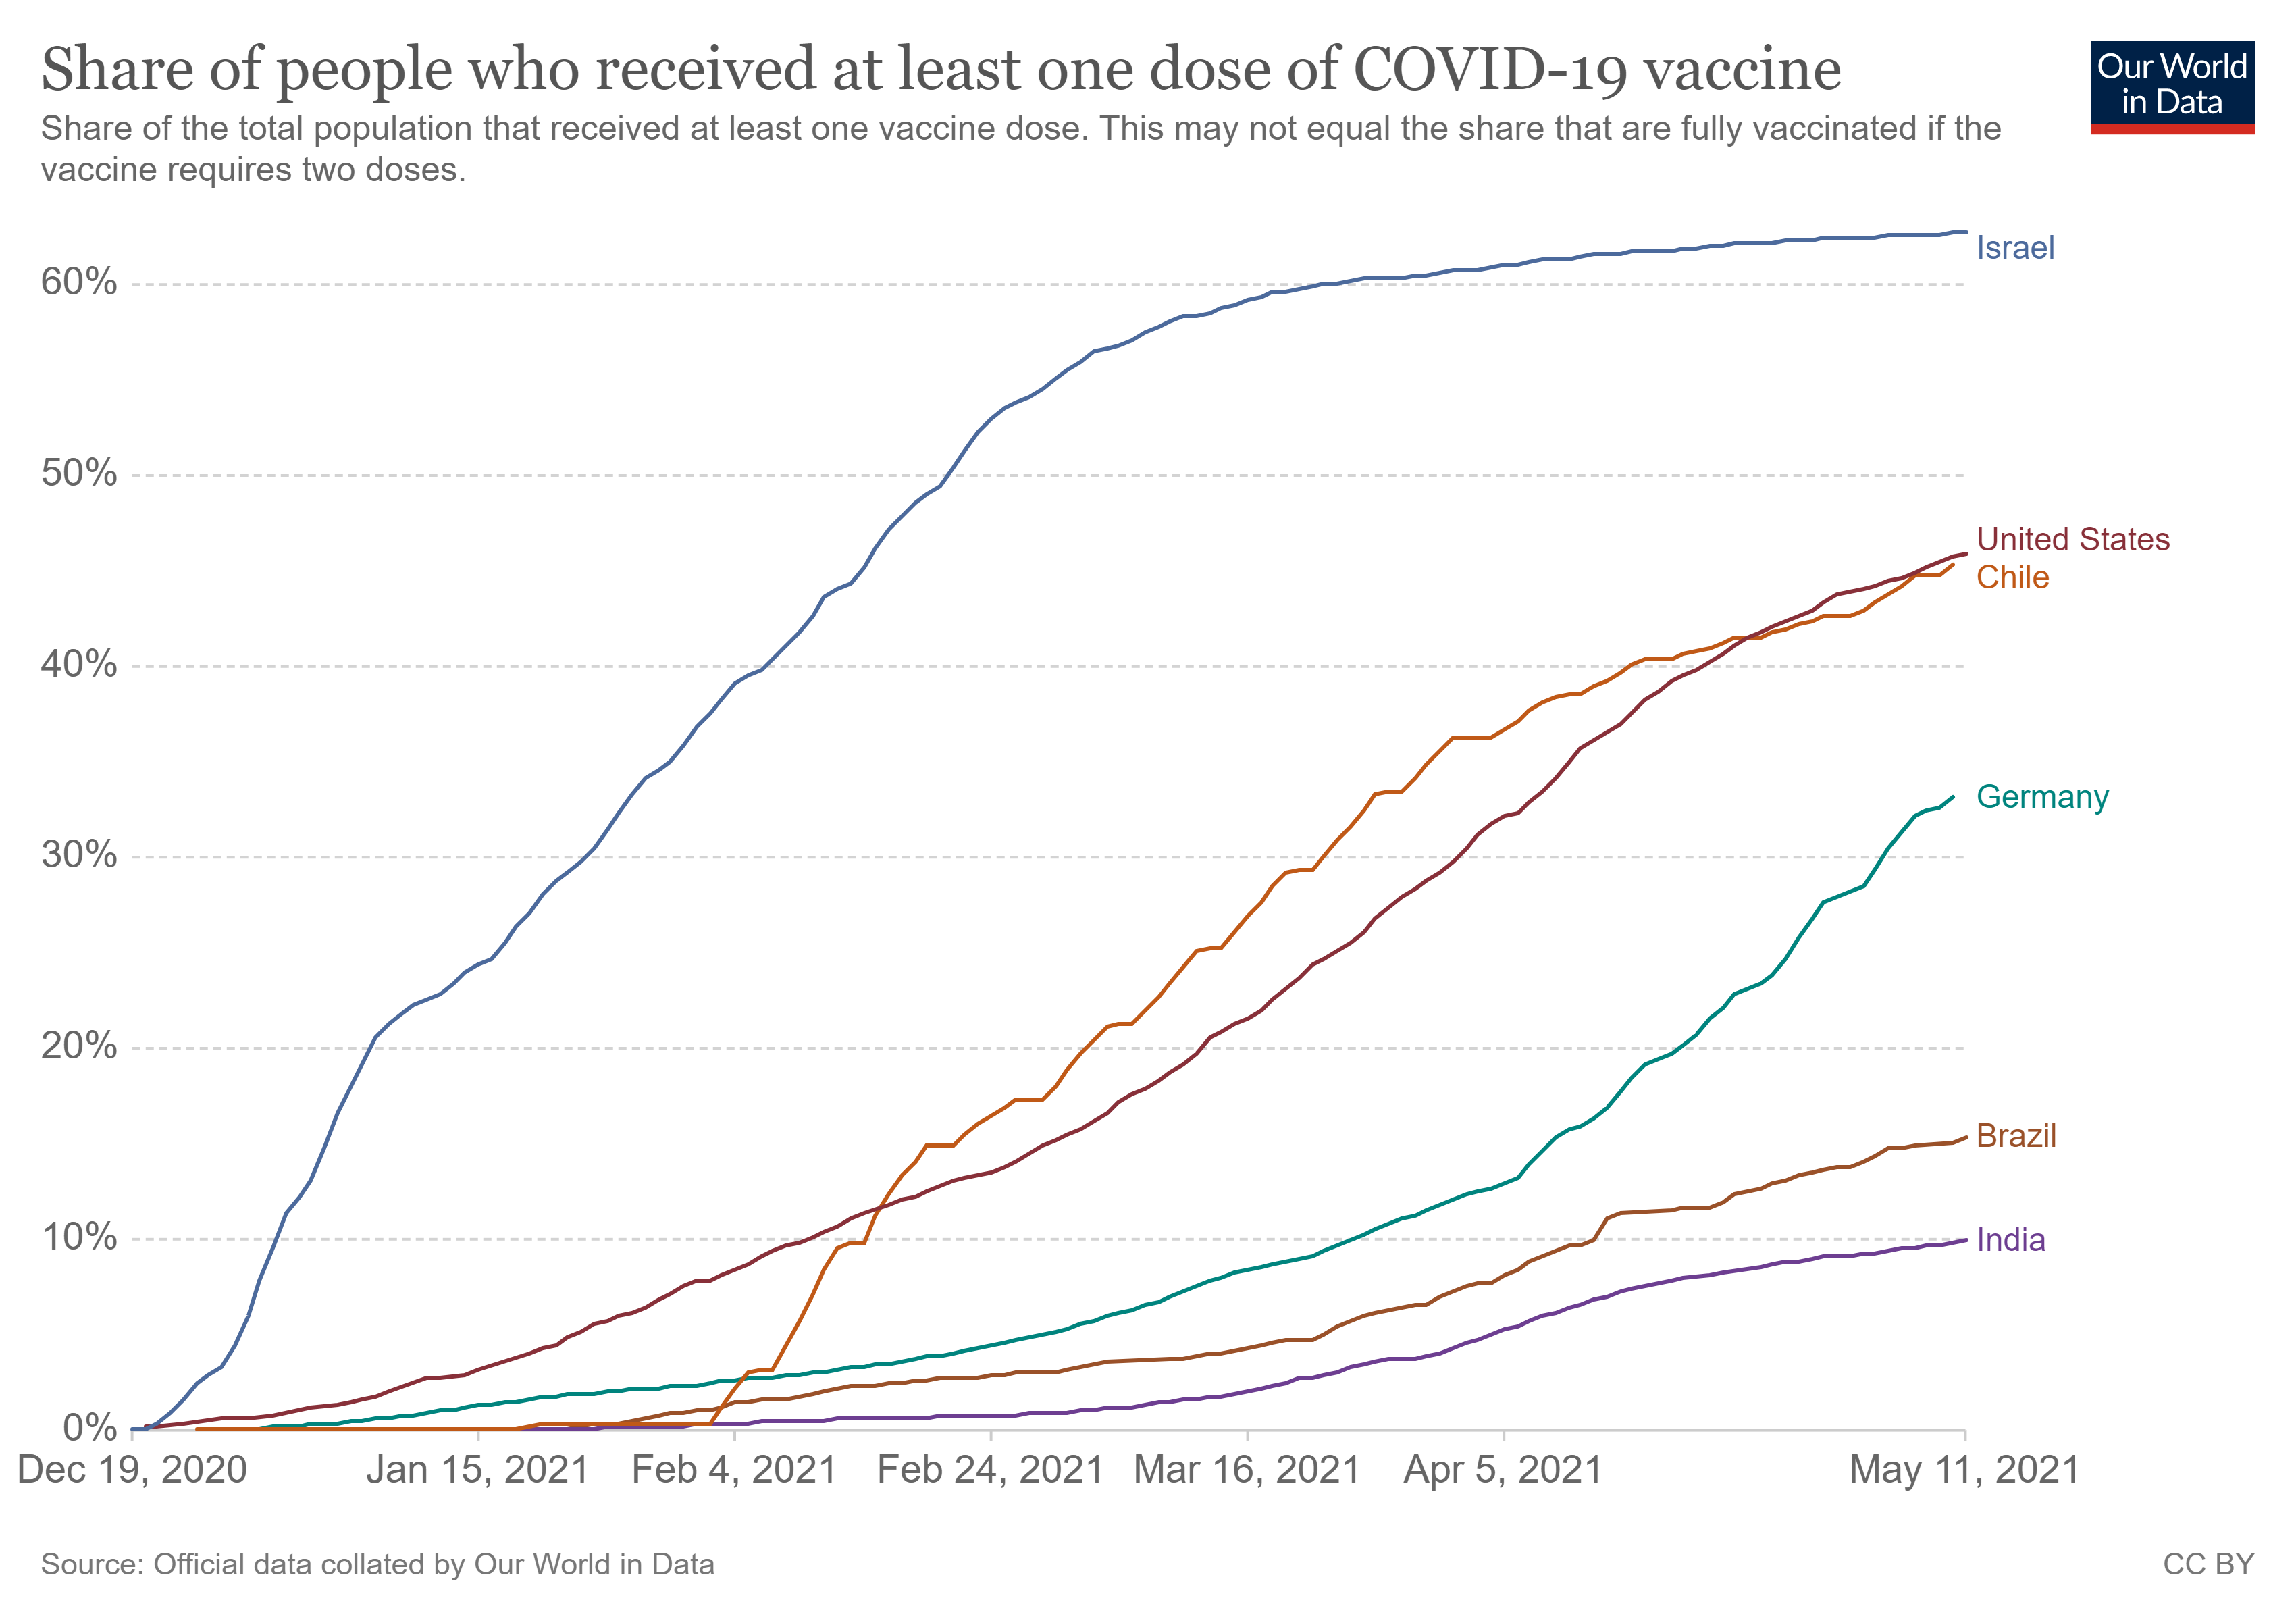
\includegraphics[width=0.45\textwidth]{vaccinepermillion.png}
    \caption{COVID-19 vaccination rate in some countries}
    \label{fig:graph3}
\end{figure}

Finally, although this topic is challenging, it allows us to combine what we learn in this course with creative thinking. We can apply the linear regression model, basic techniques of processing data in this research. We can also learn by ourselves and explore new models and algorithms in this research. Therefore, based on "interest, research value and learning exercise" these three aspects, this topic is decided.

\section{Background}
The first research is about the influencing factors of Covid-19 based on the 30 provinces in China.

It investigates multiple influencing factors, for example, the GDP of each province, the population density of each province, to find out which factors influence the spread of Covid-19. It’s conducted during the period from 2020.1.26 to 2020.2.29 with its data from Baidu and the official China government website. The result shows that the scale of the disease in the first stage, the migration rate of Wuhan’s population, and the multi-factor set of the urban population are seriously related to the expansion of the second stage of new cases.

However, there are still 3 limitations: The data is not up to date; the data is limited; the import case is not accurate, which are stated in their report, too. Therefore, inspired by its multiple factors research on Covid-19 and based on its limitation, our research steps forward to look at the data all over the world. This does not only solve the problem that data is limited and old because we use the most recent data collected by Hopkins University, which is proven to be authoritative as well. By adjusting our independent factors, the “inaccurate import data” problem is solved as well \cite{williamson2020opensafely}. In summary, we make good use of its researching process and methodology but migrate this idea to a better data source. However, apart from its researching thinking, we also integrate what we have learned in class and by ourselves into this research.

\section{Description}
We have concluded that COVID-19 may be affected by a few factors, and we have classified these factors into groups including time, virus, vaccine, government, population, and economic groups. All these groups may have more or fewer effects on virus spread. Also, different models including linear regression are all used to test for the best fit \cite{al2020optimization}. 

In this project, we define a few independent variables which are possibly related to the spread of COVID-19. For example, the date may affect the result because the overall confirmed cases will vary by date. We list more than 10 possible factors which cover different areas to figure out whether the relationship exists between these factors and COVID-19\cite{fauci2020covid,jordan2020covid}.

We have distributed our task into a few parts: Research target determination, data collection, data process, model construction, code implementation, test validation, result finalization, and report writing. We have distributed these stages of research to different group members so that we can increase efficiency and avoid time conflict.  

\section{Implementation}
\subsection{Code in R}
R has a large variety of packages that offers numerous APIs for machine learning. As the saying goes, “Don’t reinvent the wheels.”. To write the implementation of the algorithms is not feasible and our programming level is far from “invent the wheels” \cite{ihaka1996r,zeileis2001strucchange}. Meanwhile, even if we write the code to implement algorithms by ourselves, due to the shortage of time, we cannot improve it and it won’t perform as well as the APIs offered by mature advanced packages. \cite{boehmke2019hands}To balance the workload and adjust our actual ability, we choose to use built-in functions to implement our ideas \cite{crawley2012r,team2013r,lantz2013machine}.

\subsection{Models}
R has a powerful build-in function “lm()”, which we can use to construct a linear regression model. As mentioned above, we choose to use the new confirmed case rate, which is “7-day moving average of newly confirmed cases per million”, as the dependent. Then, we select a variety of independents including the rate of people that get vaccinated (represent the vaccine), stringency index (an index which can show the government regulation fight against the virus, such as knockdown and mandatory COVID-19 test), population density (reflect the difficulty that COVID-19 can spread between people), GDP per capita (reflect the economic development of this country), handwashing facilities(hand wash can prevent the spread of the virus) and human development index (reflect the medical facilities and people’s awareness of getting treatment) as an independent \cite{rath2020prediction}. 

\begin{figure}[H]
    \centering
    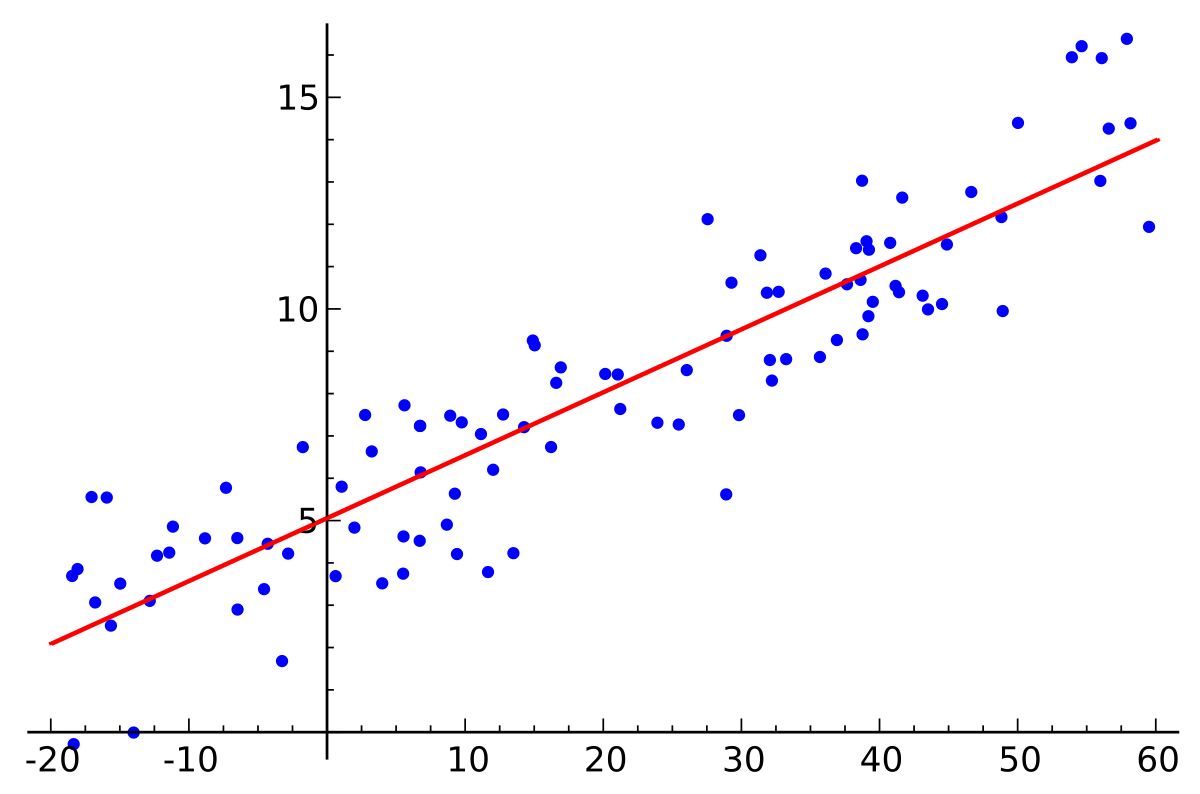
\includegraphics[width=0.45\textwidth]{samplelinearregression.png}
    \caption{A sample of linear regression}
\end{figure}

We tried multivariate linear regression to fit the data at the beginning and based on the result of the first round of model training and testing, we select the independents that have a good fit with dependent (i.e. high p-value) to do the next round of training and testing. After that, we tried to conclude and display the results \cite{ogundokun2020predictive,arino2020simple}.

Also, we tried to use multivariate polynomial regression to fit the data, and compare it with the multivariate linear regression model \cite{yan2020interpretable}. To implement the idea of a control variable, we use the same dataset and the same dependents and independents to guarantee the correctness of the result \cite{giordano2020sidarthe,fernandez2020estimating}. Similar to the multivariate linear regression model, we also select independents with a high p-value for the next round of training and testing \cite{gromping2006relative}.

\subsection{Test and Validation}
As mentioned above, four different machine learning models are implemented and finally one model are expected to be found as the best fit. To test whether our result is correct, we use split the data into training dataset and testing dataset, the “p-value” and “R-value” are calculated to evaluate the models, and after that, the model with the smallest p-value and “R-value” which is the closest to 1 has the highest accuracy.

\begin{figure}[H]
    \centering
    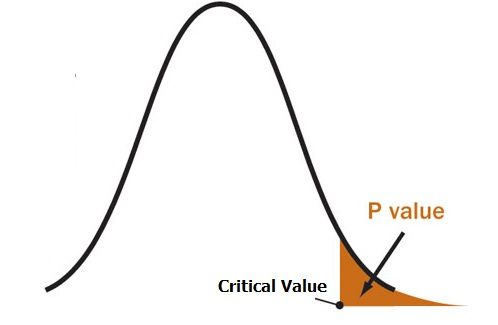
\includegraphics[width=0.45\textwidth]{pvalue.jpg}
    \caption{The visualization of p-value}
\end{figure}

\section{Data}
\subsection{Data Collection}
Data collection is an important beginning of this project, as the data will determine the goodness of fit of models and the correctness of results. Reliable sources will increase the credibility of the final result while non-official sources may lead to wrong answers. To take responsibility for humanity, we decided to only use data from official department announcements such as CDC. Data sources are attached in the appendix.

When collecting the data, we attempted a few times to get the final raw data. We tried to use a web crawler to collect the data at first, but we found that some websites do not support crawlers, or they do not provide convenient access. Then, we tried to download the statistical data manually, but we meet genuine difficulties when we tried to recognize the language different from Chinese and English. Finally, we found an organization \textit{Our World In Data}, which provides a summary of all data offered on the government or official institution website. The organization \textit{Our World In Data} provided the sources of the data, after checking, we finally determined to use the data on its GitHub repository.

\subsection{Data Selection}
The data provided by \textit{Our World In Data} is quite complete and it contains information that we do not need for analysis. Moreover, some countries with a small population are not very feasible for analysis, and part of the data in some countries is missed. To get rid of this problem, proper data selection is of vital importance, and it can also affect the result.

Because we are planning to analyze data horizontally and vertically, so we should filter the data and create a different dataset for machine learning. The dataset should be the subset of the raw table and we only keep key features that we want to analyze in the dataset. Meanwhile, we deleted countries without required features because they are not useful for the current experiment.

We initially classified the datasets into the horizontal group and vertical group. For the vertical group, we divided the data in different times, such as 2020 spring, summer, autumn, and winter, which can help us figure out the change of epidemic with time. Also, we can find how the virus is spread in specific countries and regions. For the horizontal group, we compare data from different countries. Since each country has its economic or medical situation and different policy against COVID-19. By analyzing different countries’ data, we can find the relationship between COVID-19 and country development and figure out whether a knock-down policy is necessary \cite{thompson2021interim,roser2020coronavirus}. 

\begin{figure}[H]
    \centering
    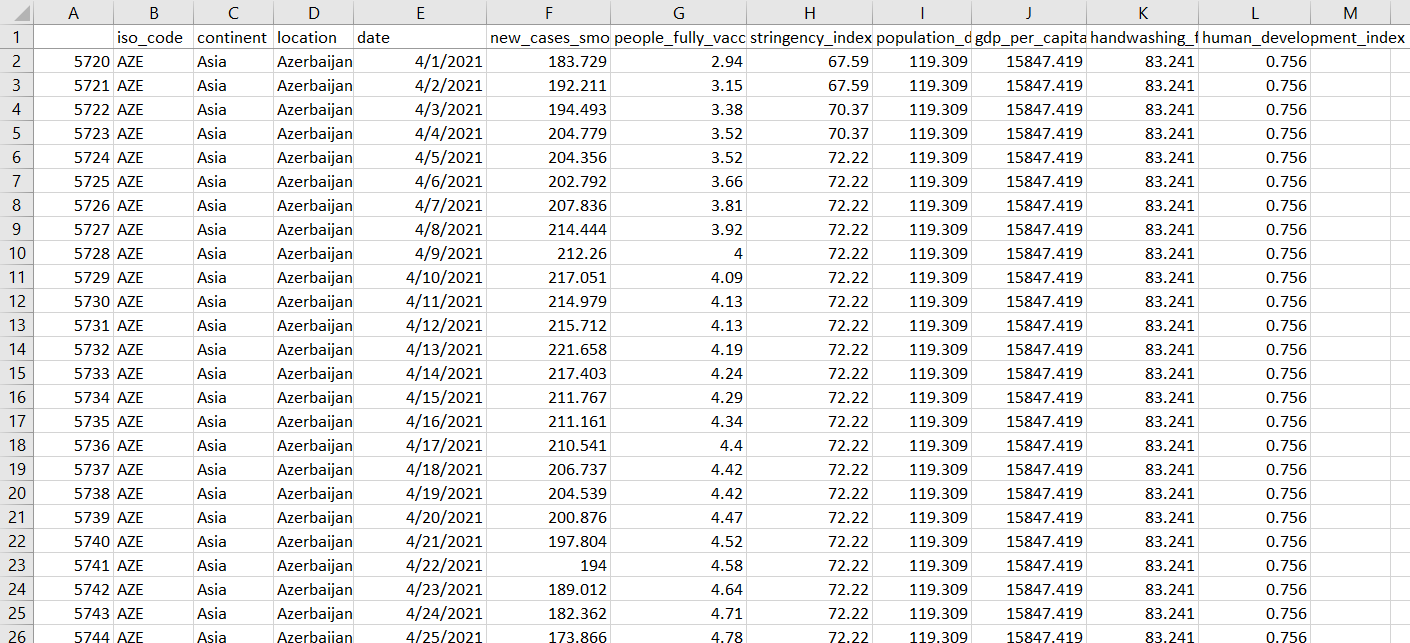
\includegraphics[width=0.45\textwidth]{selecteddata.png}
    \caption{Selected data for training}
\end{figure}

\subsection{Data Cleaning}
Sometimes, the government didn’t provide sufficient information on some holidays, but they provided it on workdays so that it is not wise to simply delete all the data of the country. Instead, we removed the rows which do not have enough data and set date as a feature so that machine learning models can understand that some rows are removed, and the models will make adjustments for these missed data.

Moreover, the raw data contains the repeated part, which may affect the result. For example, if we only want to analyze the data from different countries, the data of the continent will become useless. Therefore, we deleted these unnecessary data.

\subsection{Data Standardize}
This step is preprocessed before we use the data from Hopkins University. The feature list and the meaning of its value is listed as below.

\subsubsection{new\_cases\_smoothed\_per\_million}
\begin{itemize}
    \item \textbf{Source:} COVID-19 Data Repository by the Center for Systems Science and Engineering (CSSE) at Johns Hopkins University
    \item \textbf{Description:} New confirmed cases of COVID-19 (7-day smoothed) per 1,000,000 people
\end{itemize}

\subsubsection{new\_deaths\_smoothed\_per\_million}
\begin{itemize}
    \item \textbf{Source:} COVID-19 Data Repository by the Center for Systems Science and Engineering (CSSE) at Johns Hopkins University
    \item \textbf{Description:} New deaths attributed to COVID-19 (7-day smoothed) per 1,000,000 people
\end{itemize}

\subsubsection{people\_fully\_vaccinated\_per\_hundred}
\begin{itemize}
    \item \textbf{Source:} National government reports
    \item \textbf{Description:} Total number of people who received all doses prescribed by the vaccination protocol per 100 people in the total population
\end{itemize}

\subsubsection{total\_vaccinations\_per\_hundred}
\begin{itemize}
    \item \textbf{Source:} National government reports
    \item \textbf{Description:} Total number of COVID-19 vaccination doses administered per 100 people in the total population
\end{itemize}

\subsubsection{people\_vaccinated\_per\_hundred}
\begin{itemize}
    \item \textbf{Source:} National government reports
    \item \textbf{Description:} Total number of people who received at least one vaccine dose per 100 people in the total population
\end{itemize}

\subsubsection{stringency\_index}
\begin{itemize}
    \item \textbf{Source:} Oxford COVID-19 Government Response Tracker, Blavatnik School of Government
    \item \textbf{Description:} Government Response Stringency Index: composite measure based on 9 response indicators including school closures, workplace closures, and travel bans, rescaled to a value from 0 to 100 (100 = strictest response)
\end{itemize}

\subsubsection{population\_density}
\begin{itemize}
    \item \textbf{Source:} World Bank World Development Indicators, sourced from Food and Agriculture Organization and World Bank estimates
    \item \textbf{Description:} Number of people divided by land area, measured in square kilometers, most recent year available
\end{itemize}

\subsubsection{gdp\_per\_capita}
\begin{itemize}
    \item \textbf{Source:} World Bank World Development Indicators, source from World Bank, International Comparison Program database
    \item \textbf{Description:} Gross domestic product at purchasing power parity (constant 2011 international dollars), most recent year available
\end{itemize}

\subsubsection{handwashing\_facilities}
\begin{itemize}
    \item \textbf{Source:} United Nations Statistics Division
    \item \textbf{Description:} Share of the population with basic handwashing facilities on premises, most recent year available
\end{itemize}

\subsubsection{human\_development\_index}
\begin{itemize}
    \item \textbf{Source:} United Nations Development Programme (UNDP)
    \item \textbf{Description:} A composite index measuring average achievement in three basic dimensions of human development long and healthy life, knowledge and a decent standard of living. Values for 2019, imported from http://hdr.undp.org/en/indicators/137506
\end{itemize}

\section{Result}
\subsection{Overview}
We are trying to find out the relationships between the spread of Covid-19 and several influencing factors, especially the vaccination. So it is crucial to use proper data analysis methods and build some models to fit the conclusions. After serious consideration, we chose the linear regression model and exponential regression model. Now let me show you what we have found out \cite{perez2010genomic}.

The influencing factors are complicated and various. But we have chosen several key influencing factors, which are considered to have a great impact on the epidemic though some of them may not have significant influence in fact.

\begin{enumerate}
    \item people\_fully\_vaccinated\_per\_hundred
    \item total\_vaccinations\_per\_hundred
    \item people\_vaccinated\_per\_hundred
    \item stringency\_index
    \item population\_density
    \item gdp\_per\_capita 
    \item handwashing\_facilities
    \item human\_development\_index
\end{enumerate}

As for the value to monitor the epidemic, we chose:
\begin{enumerate}
    \item new\_cases\_smoothed\_per\_million
    \item new\_deaths\_smoothed\_per\_million
\end{enumerate}

\subsection{Vaccination and other contributing factors}
We have tried four different models, and finally, an exponential model is considered to be the most accurate and reasonable. We would like to explain it in detail.

\begin{figure}[H]
    \centering
    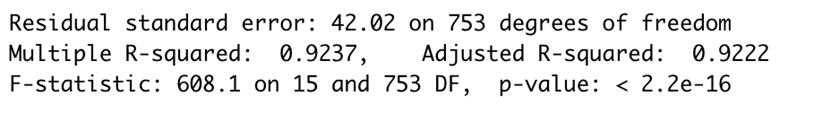
\includegraphics[width=0.45\textwidth]{errorsummary.png}
    \caption{R-square and p-value of models}
\end{figure}

As we can see, the R-squared value is close to 1 and p-value is extremely small, which have proved the accuracy of this model.

Here is the primary residual graph. The y-axis is $\frac{model\_value}{true\_value}$ and the x-axis is the time index. If most value is close to 1, the we can know the model is accurate enough. This graph is not clear enough, so we have another graph.

\begin{figure}[H]
    \centering
    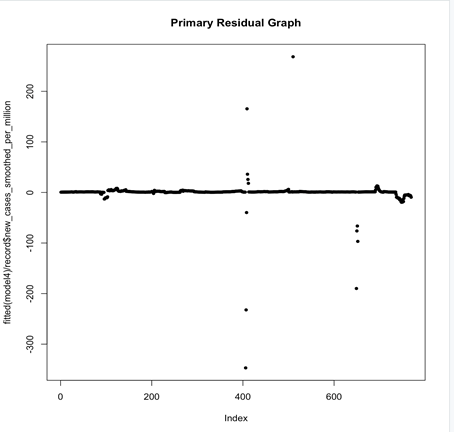
\includegraphics[width=0.45\textwidth]{primaryresidual.png}
    \caption{Accuracy Test, $\frac{model\_value}{true\_value}$}
\end{figure}

In the next graph, we remove some points that are extremely large or extremely small. And we minor 1 to every value. And we could see that most points are close to 0. So the model is relatively accurate. And it has some practical meanings for prediction.

\begin{figure}[H]
    \centering
    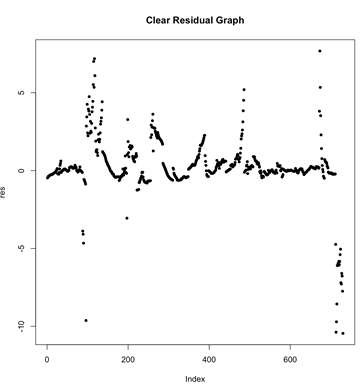
\includegraphics[width=0.45\textwidth]{clearresidual.png}
    \caption{Accuracy Test, delete outliers, $\frac{model\_value}{true\_value}$}
\end{figure}

How the factors influence the epidemic? We can find answers in the models.

\begin{figure}[H]
    \centering
    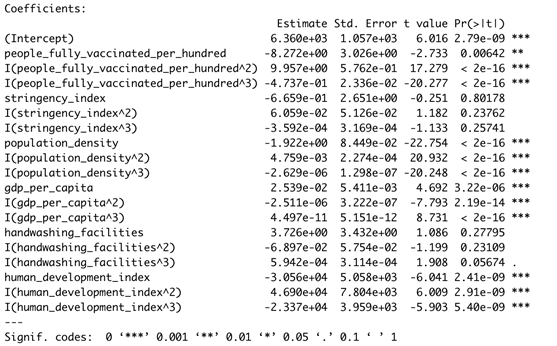
\includegraphics[width=0.45\textwidth]{rawresult.png}
    \caption{Coefficients of independents}
\end{figure}

This image shows the significance of the factors. As we can see, \textbf{handwashing\_facilities} and \textbf{stringency\_index} have low significance to the epidemic, while the others have high significance. Remove some of the factors and we have another model summary.

\begin{figure}[H]
    \centering
    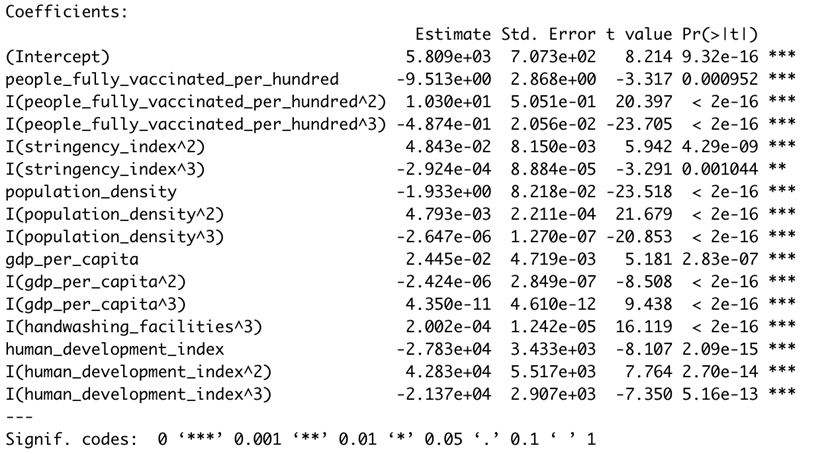
\includegraphics[width=0.45\textwidth]{improvedresult.png}
    \caption{Coefficients of independents, after the removal of low relevance factors}
\end{figure}

\subsection{Summary of program results}
After repeating experiments, we found that the spread of COVID-19 may related to with the following expressions:

%3.4.35e-11*gdp_per_capita^3 - 2.424e-6*()^2 + 2.445e-2*()
%4.-2.137e4*human_development_index^3 + 4.283e4*()^2 - 2.783e4*()
\begin{align*}
    f \propto& \Big [-0.49 \times \left(C_1\right)^3 + 10.3 \times \left(C_1\right)^2 - 9.5 \times C_1\Big ] \\
    f \propto& \Big [-2.6 \times 10^6 \times \left(C_2\right)^3 + 0.0048\times \left(C_2\right)^2 \\&- 1.93 \times \left(C_2\right) \Big ] \\
    f \propto& \Big [4.35\times 10^{-11} \times \left(C_3\right)^3 - 2.424 \times 10^{-6} \times \\&\left(C_3\right)^2 + 2.445 \times 10^{-2} \times C_3 \Big ]\\
    f \propto& \Big [-2.137\times 10^{4} \times \left(C_4\right)^3 + 4.283 \times 10^{4} \times \\&\left(C_4\right)^2 - 2.783 \times 10^{4} \times C_4 \Big ]\\
\end{align*}

In the above expressions, $f$ refers to the newly confirmed cases everyday (which can represent the spread of COVID-19) , while the $C_i$ refers to:

\begin{align*}
    C_1&=people\_fully\_vaccinated\_per\_hundred \\
    C_2&=population\_density \\
    C_3&=gdp\_per\_capita \\
    C_4&=human\_development\_index\\
\end{align*}

\section{Discussion}

In this research, we have got some results. However, due to the regression model and other possible impact features, we cannot 100 percent assert that the result is correct. Considering that the data source is reliable, and the academic integrity of the group members can be guaranteed, we can prove that the result is as correct as possible. Here are some of the possible errors that we think may affect the answer.

\begin{itemize}
    \item \textbf{Data accuracy} Some cases may be ignored by the government and they are not counted into the confirmed cases
    \item \textbf{Model Choice} The models we used may not the best model, and there may be other models which is better than current models
    \item \textbf{Change of constant values} We assume some independents as constant values, such as human development index and stringency index. However, they will change with the time.
    \item \textbf{Data selection} Because of the lack of data, only countries will complete data are selected, and this may lead to error for some developing countries.
    \item \textbf{Math error} Most of the countries have a low vaccination rate due to the large population, and it may cause math error and affect the result.
\end{itemize}

Considering the possible errors above, the result may have some differences with the reality, and we cannot fully convinced that the result is correct. More detailed and well-designed experiments required to make the final decision.
\section{Conclusion}

The development of epidemic is not influenced by one single factor, but affected by several factors. In common, more people are vaccinated or lower population density or higher gdp (more prosperous economy) or lower human\_development\_index (which may mean less educated) will contribute to the development of epidemic.

If the Hong Kong government intends to control Covid-19, I am afraid that the result will not be satisfying enough if the government only vaccines more citizens. Because according to our research, vaccination only has slight influence to the epidemic. But more importantly, as a high advanced city, control the population density (maybe control the social distance) and let more people understand the importance of it will contribute to the decrease of new cases.

\section{Appendix}
\subsection{Useful Links}
\begin{itemize}
    \item \textbf{Project Repository} \\GitHub \url{https://github.com/comp1433/Magic-Vaccine}
    \item \textbf{Data Set} \\Our World In Data \url{https://ourworldindata.org/coronavirus}
    \item \textbf{Data Set Repository} \\GitHub \url{https://github.com/owid/covid-19-data/tree/master/public/data}
    \item \textbf{Reference Source} \\Google Scholar \url{https://scholar.google.com/}
\end{itemize}
\bibliographystyle{unsrt}  
\bibliography{references}  

\end{multicols}
\end{document}